\documentclass[conference]{IEEEtran}
\IEEEoverridecommandlockouts
\usepackage{cite}
\usepackage{amsmath,amssymb,amsfonts}
\usepackage{algorithmic}
\usepackage{graphicx}
\usepackage{textcomp}
\usepackage{xcolor}
\usepackage{booktabs}
\usepackage{multirow}
\def\BibTeX{{\rm B\kern-.05em{\sc i\kern-.025em b}\kern-.08em
    T\kern-.1667em\lower.7ex\hbox{E}\kern-.125emX}}

\graphicspath{{./}}

\begin{document}

\title{Agentic Performance Boundary Discovery for Safety Assurance of
Reinforcement-Learning Autonomous Driving Policies}

\author{
\IEEEauthorblockN{Carmen L. DiMario}
\IEEEauthorblockA{\textit{Electrical Engineering and Computer Science} \\
\textit{Embry-Riddle Aeronautical University}\\
Daytona Beach, FL\\
DIMARIOC@my.erau.edu}
\and
\IEEEauthorblockN{M. \.{I}lhan Akba\c{s}}
\IEEEauthorblockA{\textit{Electrical Engineering and Computer Science} \\
\textit{Embry-Riddle Aeronautical University}\\
Daytona Beach, FL\\
akbasm@erau.edu}
}

\maketitle

\begin{abstract}
Validating reinforcement-learned (RL) policies for autonomous systems requires
characterising the Operational Design Domain (ODD), the envelope of conditions
within which a policy operates safely. Unlike programmed controllers, neural
network policies carry no explicit specification of this envelope, so it must be
discovered empirically. We present a pipeline that extends SEMBAS~\cite{b1}, a
three-phase adaptive boundary scanner, to RL policy evaluation and pairs it with
three interpretation agents that classify scan evidence, identify failure
mechanisms, and propose targeted retraining curricula. After each training phase,
the pipeline scans the scenario space, produces interpretable boundary evidence,
and generates curriculum proposals that feed directly back into training.
Deployed on CARLoS~\cite{b2}, a 2D autonomous driving simulator, the system has
guided ten training experiments spanning two RL algorithms, five curriculum
strategies, and over 1.7 million training steps. Across these experiments, the
pipeline identified a structural speed ceiling near 20~mph and, critically,
distinguished it from a soft training artifact, a finding that redirected the
investigation from training interventions toward architectural redesign. We
discuss how the boundary evidence produced by this pipeline maps to the AMLAS-RL
assurance framework~\cite{b3} and how automated boundary discovery can
accelerate safety-driven development of RL-based autonomous systems.
\end{abstract}

\begin{IEEEkeywords}
safety assurance, operational design domain, boundary scanning, reinforcement
learning, autonomous driving, AMLAS
\end{IEEEkeywords}

% =============================================================================
\section{Introduction}

Learned policies for autonomous systems introduce a fundamental assurance
challenge: unlike programmed controllers, neural network policies carry no
explicit specification of safe operating conditions. Regulators and standards
bodies increasingly require developers to characterise the
\emph{Operational Design Domain} (ODD), the set of conditions within which a
system is expected to operate safely~\cite{b7}. For RL-trained policies, this
requires empirically discovering the pass/fail boundary across a continuous
scenario space rather than deriving it analytically.

Existing approaches address related but distinct problems: falsification
searches for \emph{any} failing scenario via optimisation~\cite{b9},
adaptive stress testing finds the \emph{most likely} failure via
RL~\cite{b10}, and GP-based methods estimate performance boundaries from
sampled evaluations~\cite{b7,b8}. These produce point-failure evidence or
probabilistic envelopes, but not a dense boundary surface that supports ODD
characterisation or tracks how the boundary shifts across training iterations.
AMLAS-RL~\cite{b3} recently extended the AMLAS assurance
methodology~\cite{b4} to RL-specific challenges, but the framework requires
structured boundary evidence that existing tooling does not readily supply,
and provides no mechanism for feeding that evidence back into the training
loop.

We address this gap with a pipeline that extends SEMBAS~\cite{b1} to RL
policy evaluation and pairs it with interpretation agents that close the loop
between boundary discovery and retraining. To our knowledge, this is the first
system to (a)~produce a dense, comparable ODD boundary surface across RL
training iterations, and (b)~automatically translate that boundary evidence
into targeted curriculum proposals without manual intervention. The pipeline's
core value is not only in finding failures, but in characterising \emph{what
kind} of boundary exists: soft and addressable by further training, or
structural and requiring architectural change. Our contributions are:

\begin{itemize}
\item An RL-specific deployment of SEMBAS~\cite{b1} on CARLoS~\cite{b2}
with six boundary metrics that can be tracked and compared across training
checkpoints.
\item Three interpretation agents (Policy Down-Selection, Failure Mechanism
Analysis, and Boundary-Aware Retraining Planning) that automate post-scan
analysis and generate actionable curriculum proposals.
\item A ten-experiment deployment demonstrating the pipeline's ability to
distinguish a structural ODD boundary from a soft training artifact, and to
direct the investigation accordingly across two RL algorithms and five
curriculum strategies.
\item A step-level diagnostic methodology that traces the identified structural
limit to speed-steering coupling in the CARLoS dynamics, grounding the
boundary evidence in a concrete physical mechanism.
\end{itemize}

% =============================================================================
\section{System Overview}

\subsection{CARLoS Simulation Environment}

CARLoS~\cite{b2} is a 2D top-down driving simulator in which a vehicle
navigates a curved lane with static obstacles. Episodes terminate via
\texttt{truncated} (200-step survival $=$ PASS) or \texttt{terminated}
(collision / lane exit / stop $=$ FAIL). The scenario space is
three-dimensional:
\begin{equation}
\mathbf{x} \in [0,1]^3 \;\leftrightarrow\;
\bigl(
  \underbrace{x_0}_{\text{lane width}\,[10,14]\,\text{ft}},\;
  \underbrace{x_1}_{\text{obstacles}\,[4,10]},\;
  \underbrace{x_2}_{\text{speed}\,[10,75]\,\text{mph}}
\bigr).
\end{equation}
The agent observes 12 distance sensor readings (range 120~ft,
$\Delta t = 0.1$~s). The baseline policy is trained via PPO~\cite{b5} through
a three-stage curriculum (Easy, Medium, Hard; 282,272 total steps).

\subsection{SEMBAS Boundary Scanner}

SEMBAS~\cite{b1} operates in three sequential phases over the normalised
scenario space $[0,1]^3$.

\textbf{Phase~1: LHS Seeding.} Latin Hypercube Sampling draws $N_{\text{seed}}$
scenarios to maximally cover the space. Each is evaluated and labelled
PASS/FAIL.

\textbf{Phase~2: Binary Bisection.} For each adjacent PASS/FAIL pair from
Phase~1, bisection along the connecting segment locates the boundary crossing
to within tolerance $\epsilon$.

\textbf{Phase~3: Boundary Walking.} Each bisection seed walks along the
estimated boundary tangent, using localised bisection at each step to stay
on the surface and densify geometry.

Determinism is enforced by deriving a per-scenario RNG seed from the master
seed and scenario parameters, so each (lane width, obstacle count) pair
receives a reproducible obstacle layout across repeated queries.

\subsection{Boundary Metrics}

We compute six metrics per scan: (1)~Hausdorff distance, the worst-case
boundary shift between checkpoints; (2)~Chamfer distance, the mean shift;
(3)~Boundary Surface Error (BSE); (4)~near-boundary fail probability;
(5)~boundary drift along the speed axis; and (6)~pass-region coverage.

\subsection{Interpretation and Retraining Agents}

The key distinction of our approach is that boundary evidence does not sit
idle; three agents process each scan automatically and feed their outputs
back into the training loop, without requiring manual analysis between
iterations.

\textbf{Policy Down-Selection Agent.} Rather than scanning every checkpoint,
this agent ranks candidates by a composite boundary metric score and selects
the most informative one for full scanning. Applied across Stage~1--3
checkpoints, it identified Stage3-Hard-282k as the strongest baseline,
reducing scan overhead while preserving coverage.

\textbf{Failure Mechanism Analyst.} Classifies fail points by proximity to
the boundary and speed regime, distinguishing sharp structural boundaries from
diffuse transition zones. Across our experiments, Type~B failures (nearest
boundary point ${<}0.1$ normalised) account for 63.7\% of all failures,
evidence of a sharp, consistent boundary rather than noisy stochastic
behaviour.

\textbf{Boundary-Aware Retraining Planner.} Translates boundary geometry
directly into curriculum proposals ranked by projected pass-region coverage
gain. The top-ranked proposal in our initial deployment projected coverage
growth from 12.77\% to 23.17\%, providing the concrete training targets for
the subsequent experiments.

\begin{figure*}[t]
\centerline{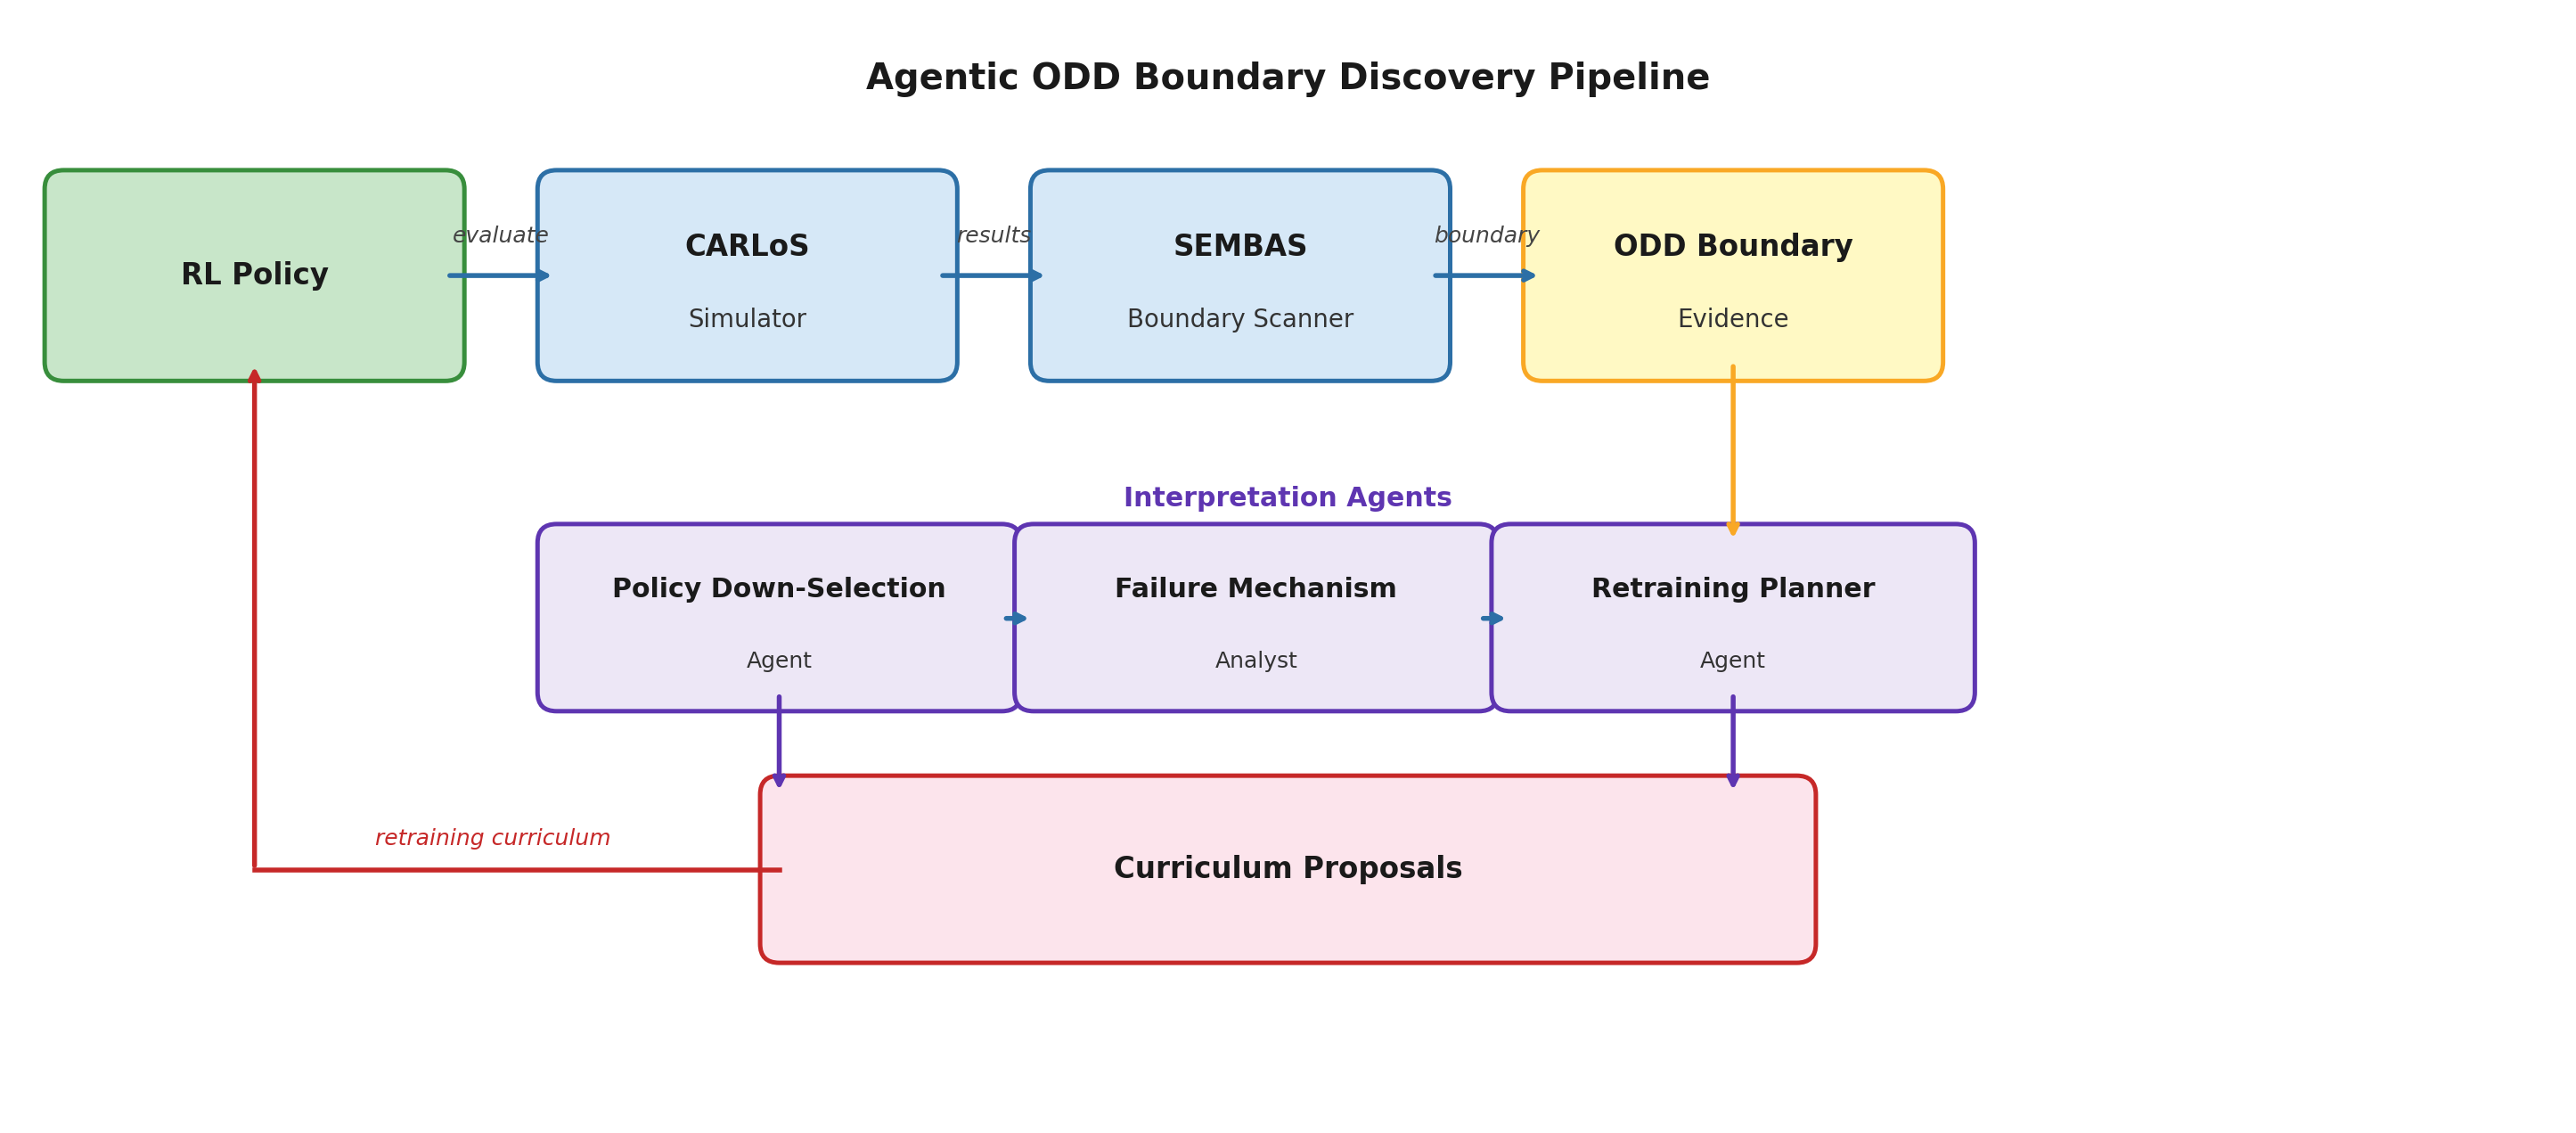
\includegraphics[width=\textwidth]{fig1_system_diagram.png}}
\caption{Overview of the agentic boundary discovery pipeline. The RL policy
is evaluated by SEMBAS to produce ODD boundary evidence, which three
interpretation agents process automatically to classify failures, rank
checkpoints, and propose retraining curricula, closing the loop back into
training without manual intervention.}
\label{fig:system}
\end{figure*}

% =============================================================================
\section{Pipeline in Action: Evidence from Ten Experiments}

\subsection{Boundary Scans Across Ten Experiments}

The following results illustrate the pipeline operating as intended: each
scan produces structured boundary evidence, the agents interpret it, and the
interpretation drives the next training decision. The value is not in any
single experiment's outcome, but in the system's ability to tell the
difference between a policy that needs more training and one that has hit a
wall the current architecture cannot overcome.

\begin{table}[htbp]
\caption{SEMBAS results across completed training experiments. Speed ceiling
is the maximum speed of any PASS point. Hausdorff is relative to Stage3.}
\label{tab:results}
\begin{center}
\resizebox{\columnwidth}{!}{%
\begin{tabular}{lccc}
\hline
\textbf{Experiment} & \textbf{Pass\%} & \textbf{Speed Ceil.} & \textbf{Hausdorff} \\
\hline
Stage3-282k (PPO baseline)        & 40.3\% & 19.8~mph & --    \\
Stage4 +30k (biased curriculum)   & 40.3\% & 19.8~mph & 0.024 \\
Stage4b +150k (biased curriculum) & 38.8\% & 19.8~mph & 0.029 \\
ExpA: high LR + entropy (PPO)     & 40.7\% & 19.8~mph & 0.024 \\
ExpB: staged speed curriculum     & 40.5\% & 19.8~mph & 0.037 \\
ExpC: reward shaping (PPO)        & 38.8\% & 19.8~mph & 0.023 \\
SAC + speed observation, 500k     & 41.1\% & 19.4~mph & 0.246 \\
SPS-PPO, +500k steps              & 39.7\% & 19.4~mph & 0.024 \\
ExpD: speed obs + SPS + bridge    & 42.5\% & 17.1~mph & 0.112 \\
ExpE: 300~ft sensors + speed obs  & 36.3\% & 19.2~mph & 0.338 \\
\hline
\end{tabular}
}
\end{center}
\end{table}

Pass rates cluster at $40 \pm 1$\% and the speed ceiling is invariant at
approximately 19--20~mph across all experiments (Fig.~\ref{fig:comparison}).
The SAC experiment (Soft Actor-Critic~\cite{b6} with speed appended to the
12D observation) produced a qualitatively different boundary shape (Hausdorff
0.246 vs.\ 0.023--0.037 for PPO variants), confirming that a different policy
was learned, yet the ceiling did not move. ExpD (speed observation co-trained
with a Speed-Proportional Steering wrapper, warm-started via weight surgery on
Stage3) produced a slight regression to 17.1~mph (Hausdorff 0.112), consistent
with weight surgery disrupting the Stage3 representation before the policy
could recover high-speed behaviour. ExpE extended sensor range to 300~ft,
normalised observations to $[0,1]$, and trained from a fresh curriculum; the
ceiling held at 19.2~mph with a substantially different boundary geometry
(Hausdorff 0.338), the largest shape shift observed across all experiments,
confirming the physical constraint hypothesis: additional reaction time does
not overcome the steering-authority limit at speed.

\begin{figure*}[t]
\centerline{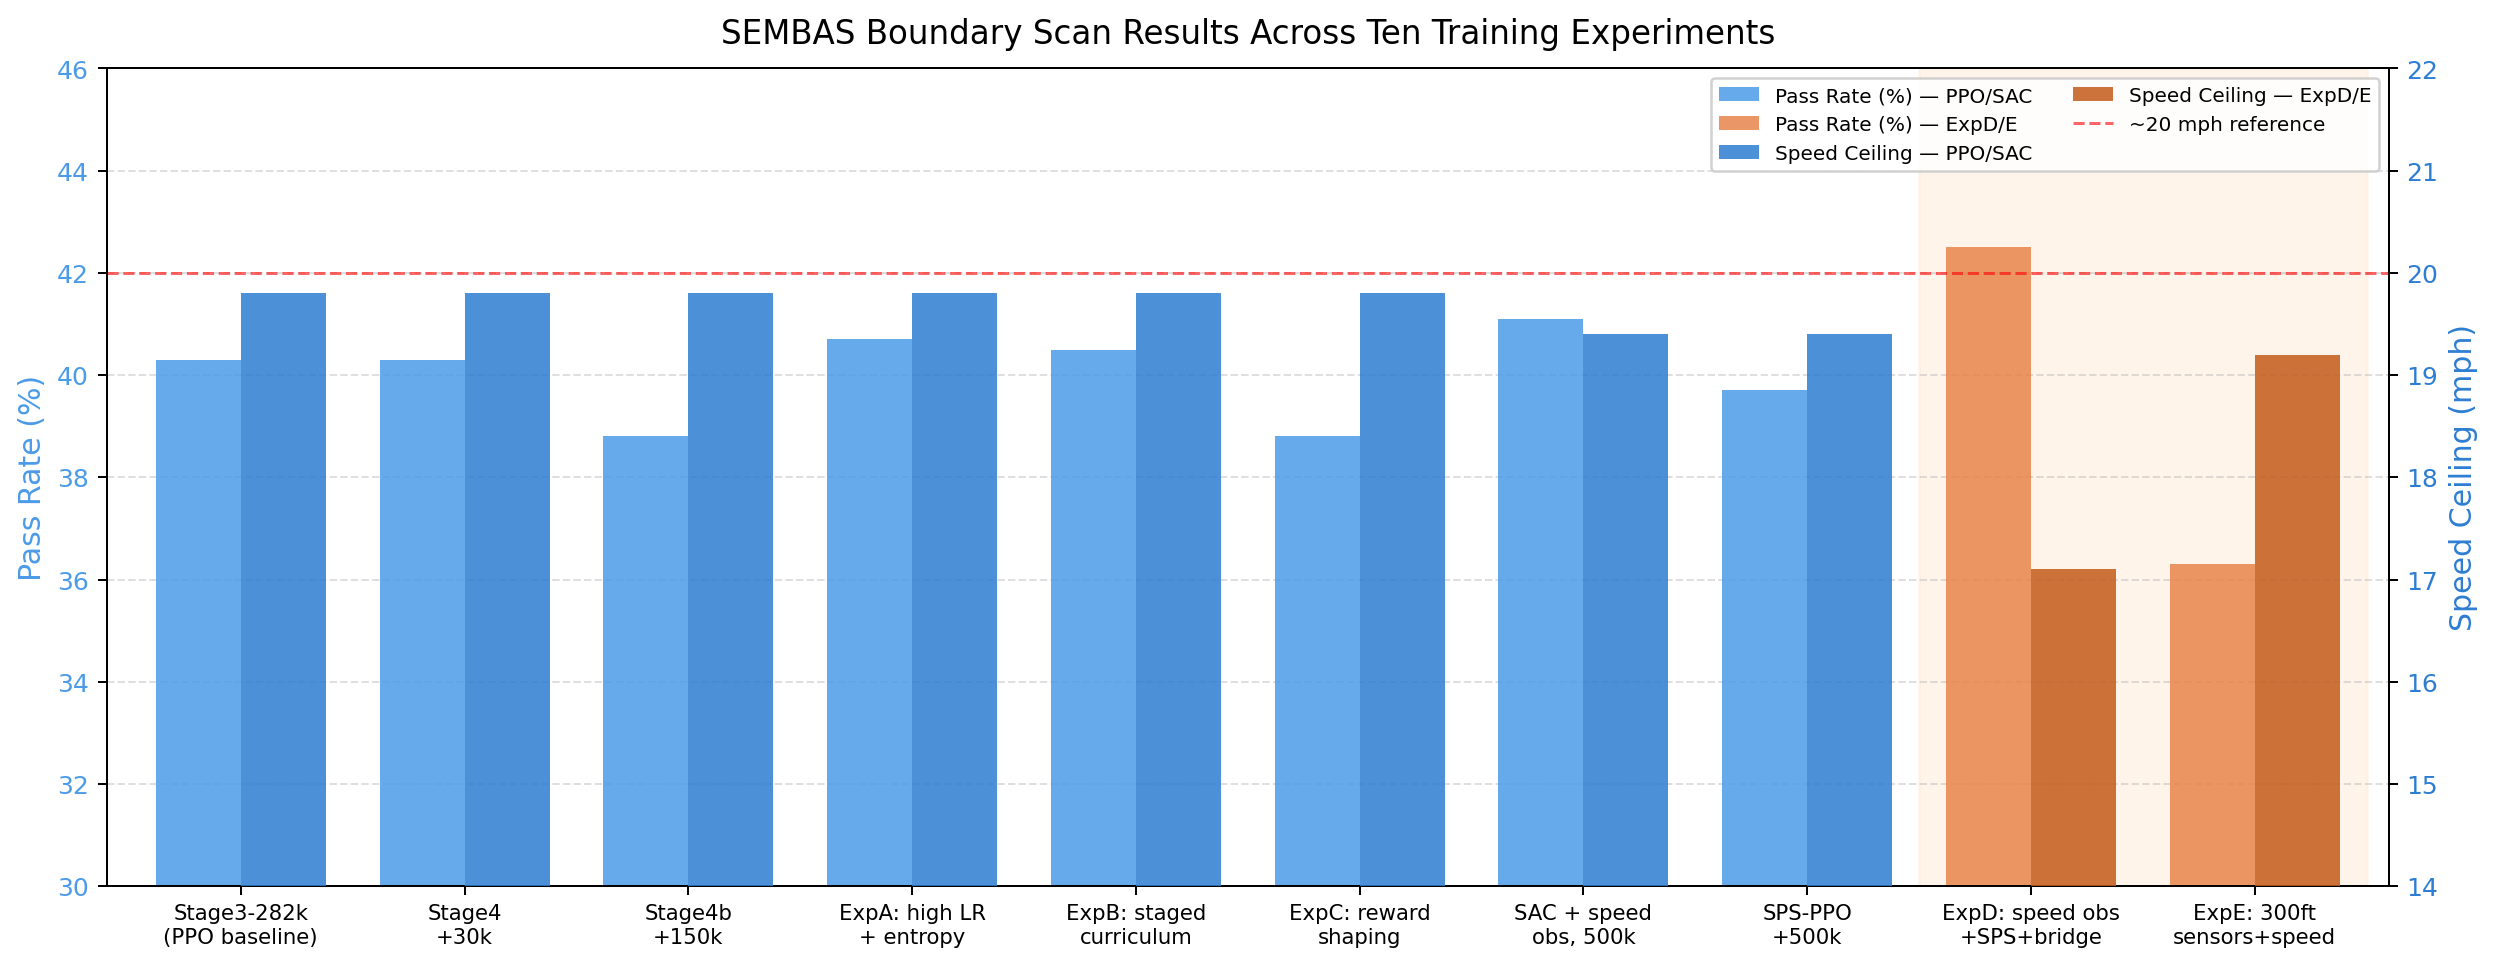
\includegraphics[width=\textwidth]{fig2_experiment_comparison.png}}
\caption{Pass rate and speed ceiling across all completed experiments. The
ceiling holds near 20~mph across varied algorithms, curricula, and observation
spaces.}
\label{fig:comparison}
\end{figure*}

\subsection{Root Cause Diagnostic}

The persistence of the ceiling across ten experiments motivates step-level
episode analysis. We instrument an episode tracer logging sensor readings,
actions, and vehicle state at each timestep for episodes at 15, 20, 30, and
40~mph. All failures above 20~mph are out-of-lane, not collision.
Table~\ref{tab:diag} shows the mechanism: perceived obstacle proximity
increases with speed because the vehicle covers more ground per timestep. At
40~mph the policy reaches maximum steering from step~2 and cannot recover.

\begin{table}[htbp]
\caption{Step-1 sensor reading and steering action by initial speed.}
\label{tab:diag}
\begin{center}
\begin{tabular}{|c|c|c|}
\hline
\textbf{Speed} & \textbf{Min sensor (step 1)} & \textbf{Steering (step 1)} \\
\hline
15~mph & 2.63~ft & $-$0.30~rad \\
20~mph & 2.49~ft & $-$0.43~rad \\
30~mph & 2.22~ft & $-$0.81~rad \\
40~mph & 2.02~ft & $-$1.00~rad (max) \\
\hline
\end{tabular}
\end{center}
\end{table}

At speed $v$, the step-1 sensor reading is approximately $s_0 - v\,\Delta t$
because the vehicle has already closed distance to the obstacle. Without speed
in the observation, the policy cannot scale its steering response
appropriately. Adding speed to the observation (SAC) did not resolve this
within 500k steps, and a Speed-Proportional Steering wrapper applied at
inference also produced no improvement, because the policy must co-learn to
brake in high-speed scenarios.

\subsection{Mapping to AMLAS-RL}

The invariance of the speed ceiling across ten interventions constitutes
preliminary evidence of a structural ODD boundary at $x_2 \leq 0.15$
(${\leq}19.75$~mph). Under AMLAS-RL~\cite{b3}, this contributes to three
evidence items: ODD characterisation from consistent boundary geometry;
learning sufficiency evidence from Hausdorff stability across eight PPO/SAC
variants; and a safety argument that higher-speed operation requires a
fundamental architectural change (e.g., recurrent policy, richer simulation
dynamics, or explicit braking authority) rather than additional training steps
or observation augmentation alone.

% =============================================================================
\section{Future Directions}

This is precisely where the pipeline's value becomes concrete. After ten
experiments, the boundary evidence accumulated by SEMBAS (not intuition or
training curves alone) is what allowed us to conclude that the ceiling is
structural rather than soft. That diagnosis is now directing the investigation
toward architectural interventions that training-only approaches would have
continued to pursue indefinitely. Current directions include:

\textbf{Recurrent policy architectures.} An LSTM or GRU policy can integrate
temporal velocity cues and learn to co-schedule steering and braking over
multiple timesteps, which a feedforward policy cannot.

\textbf{Formalising AMLAS-RL evidence mapping.} The ten-experiment scan corpus
provides a concrete starting point for populating the assurance argument
structures defined in AMLAS-RL~\cite{b3}, mapping boundary evidence to
specific safety claims.

\textbf{Higher-dimensional scenario spaces.} Extending the scenario to include
weather, sensor noise, and traffic density will stress-test whether the agentic
pipeline remains tractable as dimensionality grows.

% =============================================================================
\begin{thebibliography}{00}

\bibitem{b1}
J.~M. Thompson, Q.~Goss, and M.~\.{I}. Akba\c{s}, ``A strategy for boundary
adherence and exploration in black-box testing of autonomous vehicles,'' in
\textit{Proc. IEEE Int. Conf. Mobility, Operations, Services and Technologies
(MOST)}, 2023, pp. 193--201, doi: 10.1109/MOST57249.2023.00028.

\bibitem{b2}
A.~Summer, J.~M. Thompson, and M.~\.{I}. Akba\c{s}, ``CARLoS: Customizable
autonomy research low-fidelity simulator for safety testing of agents,'' in
\textit{Proc. IEEE World Forum on Public Safety Technology (WF-PST)}, 2025.

\bibitem{b3}
C.~C. Imrie, I.~Stefanakos, S.~Shahbeigi, R.~Hawkins, and S.~Burton,
``Assuring the safety of reinforcement learning components: AMLAS-RL,''
\textit{arXiv:2507.08848}, 2025.

\bibitem{b4}
R.~Hawkins, C.~Paterson, C.~Picardi, Y.~Jia, R.~Calinescu, and I.~Habli,
``Guidance on the assurance of machine learning in autonomous systems
(AMLAS),'' \textit{arXiv:2102.01564}, 2021.

\bibitem{b5}
J.~Schulman, F.~Wolski, P.~Dhariwal, A.~Radford, and O.~Klimov, ``Proximal
policy optimization algorithms,'' \textit{arXiv:1707.06347}, 2017.

\bibitem{b6}
T.~Haarnoja, A.~Zhou, P.~Abbeel, and S.~Levine, ``Soft actor-critic:
Off-policy maximum entropy deep reinforcement learning with a stochastic
actor,'' in \textit{Proc. ICML}, 2018.

\bibitem{b7}
F.~Batsch, A.~Daneshkhah, M.~Cheah, S.~Kanarachos, and A.~Baxendale,
``Performance boundary identification for the evaluation of automated vehicles
using Gaussian process classification,'' in \textit{Proc. IEEE ITSC}, 2019.

\bibitem{b8}
J.~Norden \textit{et al.}, ``High-dimensional functional boundaries search
for deviation-robust testing of autonomous driving systems,''
\textit{Accident Analysis \& Prevention}, 2025.

\bibitem{b9}
T.~Dreossi \textit{et al.}, ``VerifAI: A toolkit for the formal design and
analysis of AI-based systems,'' in \textit{Proc. CAV}, 2019.

\bibitem{b10}
A.~Corso, R.~Moss, M.~Koren, R.~Lee, and M.~J. Kochenderfer, ``A survey of
algorithms for black-box safety validation of cyber-physical systems,''
\textit{J. Artificial Intelligence Research}, vol. 72, pp. 377--428, 2021.

\end{thebibliography}

\end{document}
